\section{Evaluation}
\label{sec:eval}
%In this section, we introduce the experimental setup
%and analyze the performance of different models.
%All of the data and source code
%can be downloaded from http://202.120.38.146/sumrep.}.

\subsection{Datasets}
CNN/Daily Mail~\cite{HermannKGEKSB15}
\footnote{\url{https://cs.nyu.edu/~kcho/DMQA/}} 
is a popular summarization dataset, 
which contains news articles paired with summaries.
There are 286,817 training pairs,
13,368 validation pairs and 11,487 test pairs.
\tabref{tab:example} shows an example pair from training data.
We follow See~\cite{SeeLM17} in data preprocessing and use 
the non-anonymized version, which fills in the blanks with answer named entities.
%We show an example of such pairs in \tabref{tab:gold_a}.


\subsection{Model Parameters and Evaluation Metrics}
\label{sec:expset}
All the competing models contain $8$ convolutional layers in
both encoders and decoders, with kernel width of $3$.
For each convolutional layer, 
we set the hidden state size to $512$ and the embedding size to $256$.
%To alleviate overfitting,
We apply a \textit{dropout} ($p=0.2$) layer to 
all convolutional and fully connected layers.
Similar to \cite{gehring2017convs2s},we use Nesterov's
%DIF < accelerated gradient method \cite{SutskeverMDH13} with gradient clipping $0.1$ \cite{PascanuMB13}, momentum $0.99$,
accelerated gradient method \DIFaddbegin \DIFadd{\mbox{%DIFAUXCMD
\cite{SutskeverMDH13} }\hspace{0pt}%DIFAUXCMD
}\DIFaddend with gradient clipping $0.1$ \DIFaddbegin \DIFadd{\mbox{%DIFAUXCMD
\cite{PascanuMB13}}\hspace{0pt}%DIFAUXCMD
}\DIFaddend , momentum $0.99$,
%DIF > accelerated gradient method with gradient clipping $0.1$, momentum $0.99$,
and initial learning rate $0.2$.
Training terminates when learning rate $\le 10e$-$5$.
Beam size $b=5$ at test time.

We set the threshold $sz$ to $3$, 
because nearly $90\%$ 
of sections are with length$>=$3.
We set $n$ (Equation (\ref{eq:s})) to $5$,
since less than $5\%$ of reference summaries have
the LCS of less than $5$.
We use the following evaluation metrics:
\itemsep0em
\begin{itemize}

\item \textbf{ROUGE} scores (F1), including ROUGE-1 (R-1), ROUGE-2 (R-2) and
ROUGE-L(R-L)~\cite{rouge-a-package-for-automatic-evaluation-of-summaries}.
%ROUGE-2 is the most popular metric for summarization.

\item \textbf{Repeatedness} (Rep) includes N-gram repeatedness, sentence repeatedness
and total repeatedness. 
N-gram or sentence repeatedness is the percentage of repeated N-grams 
or sentences in a summary:

\begin{equation}
\small Rep = \frac{n}{N}
\end{equation}
where $n$ is the number of repeated N-grams or sentences, 
$N$ is the total number of N-grams or sentences in a summary.
We use \textit{sim} in \eqnref{eq:s} to
%estimate whether an N-gram or a sentence repeats.
identify repetitive sentences.
Total repeatedness (Algorithm \ref{alg:red}) is a comprehensive score that unifies N-gram and sentence repeatedness.

\begin{algorithm}[th]
\caption{Calculation of Total Repeatedness}
\small
\label{alg:red}
\textbf{Input}: a sentence set $s = {s_{1}, s_{2},...,s_{n}}$\\
%\textbf{Parameter}: Optional list of parameters\\
\textbf{Output}: Total repeatedness percentage $p$
\begin{algorithmic}[1] %[1] enables line numbers
\STATE Let $total$ be the sum of lengths of the sentences in $s$.
\STATE $n \leftarrow total$
\STATE $overlap \leftarrow 0$
\WHILE{$n \geq 3$}
\STATE The lengths of LCS between two sentences from $s$ comprise a length set $L$.
\STATE $n \leftarrow \max(L)$.
\STATE Find a substring $b$ with length $n$ that appears most frequently in $s$.
\STATE Let $k$ be the frequency that $b$ appears in $s$.
\STATE $overlap \leftarrow overlap + k\cdot n$
\STATE Remove every appearance of substring $b$ from sentences in $s$.
\ENDWHILE
\STATE $p \leftarrow overlap/total$
\STATE \textbf{return $p$} 
\end{algorithmic}
\end{algorithm}

\item \textbf{Readability} (Readable) is human evaluation, 
the percentage of
\textit{readable} sentences in summaries.
%Sentences are more complete than segment so that they can
%be evaluated easily.
Here we score sentences instead of segments because segments often have
insufficient information to determine readability.
A \textit{readable} sentence is free of grammatical and 
factual errors, 
and is logically consistent with source document.
%\begin{equation}
%Correct = \frac{n_{ct}}{N_{all}}
%\end{equation}
%where $n_{ct}$ and $N_{all}$ denotes
%the number of \textit{correct} sentences and all sentences 
%in a summary respectively.
\end{itemize}

We use \textit{readability} to complement ROUGE scores 
since Yao~\DIFdelbegin \DIFdel{\mbox{%DIFAUXCMD
\cite{Yao} }\hspace{0pt}%DIFAUXCMD
}\DIFdelend \DIFaddbegin \DIFadd{\mbox{%DIFAUXCMD
\cite{YaoWX17} }\hspace{0pt}%DIFAUXCMD
}\DIFaddend showed that the standard 
ROUGE scores cannot capture grammatical or factual errors. 
We randomly sample 300 summaries generated by each model
and manually check their readability. 
%This is a simplified human-evaluation of summarization,  
%It is easier to do and more reliable than other human-evaluations
%since we only need to check whether the sentences in a summary are \textit{correct} or not.
This metric is more objective and practical compared with
scoring the whole summary \cite{D18-1205}, since we only need 
to determine whether a sentence is {\em readable} or not.
Each sentence is scored by two judges proficient in English. 
The Cohen's Kappa coefficient between them is $0.83$, 
indicating agreement. Here we use the average annotation score.
%The score of each model is the proportion
%of {\em readable} sentences in total.

\subsection{Baselines}
%In this experiment, we take vanilla CNN seq2seq model as our basic model,
We take vanilla CNN seq2seq model as our basic model,
%because it is a more powerful toolkit for sequence modeling than
%recurrent seq2seq models~\cite{bai2018empirical}.
because it is fast and enjoys the best accuracy among
the other vanilla RNN seq2seq models~\cite{bai2018empirical,gehring2017convs2s}.
We did not implement the repetition reduction methods 
on top of SOTA seq2seq models,
because the tricks employed in these SOTA models may 
interact with the repetition reduction methods 
and impact the evaluation results (ROUGE), which complicate the analysis.
%DIF < \KZ{Be careful with what you say here, which might conflict with 
%DIF < the statements in intro.}
\DIFdelbegin \DIFdel{Our main purpose is to evaluate }\DIFdelend \DIFaddbegin \DIFadd{Our evaluation mainly compares }\DIFaddend the effectiveness of \DIFdelbegin \DIFdel{repetition reduction
on CNN-based models }\DIFdelend \DIFaddbegin \DIFadd{different repetition reduction techniques,
in terms of all three metrics above. If these methods were
applied on top of more advanced models such as PtGen (effectively it is CNN with mechanism that cannot reduce repetition), 
the room for improvement on the ROUGE score will be
very limited because the advanced models already achieves very high ROUGE scores for any abstractive
summarization techniques. 
Consequently, the differences in ROUGE scores by these repetition reduction techniques will be
indistinguishable. 
As shown in }\tabref{tab:compete_exp}\DIFadd{, after reducing repetition, the summary becomes better
but the ROUGE score is not improved. 
Hence, in this work, we choose to implement these methods (}\tabref{tab:eval_main}\DIFadd{) on top of vanilla CNN model}\DIFaddend .
We construct \DIFdelbegin \DIFdel{several baselines  
(}%DIFDELCMD < \tabref{tab:baselines}%%%
\DIFdel{) 
}\DIFdelend \DIFaddbegin \DIFadd{seven baselines  
}\DIFaddend %by converting some of RNN-based models to
%CNN seq2seq architectures, 
by converting
repetition reduction techniques developed on RNN seq2seq models to their
counterparts on CNN seq2seq models,
%\KZ{How can u convert RNN models to CNN models? I think what you mean is
%repetition reduction techniques developed on RNN models to their counterparts on CNN models.} 
to be fair.
%DIF > Details are illustrated in Introduction. 
%DIF > \KZ{Not sure what you mean by
%DIF > illustrated in Introduction... It's a bit weird to refer back to previous 
%DIF > sections.}

\begin{itemize}

\item \textbf{CNN}: Convolutional seq2seq model~\cite{gehring2017convs2s} 

\item \textbf{ITA}: Intra-temporal attention~\cite{NallapatiZSGX16} 

\item \textbf{ITDA}: Intra-temporal attention and intra-decoder attention~\cite{PaulusXS17,FanGA18}

\item \textbf{COV}: Coverage mechanism~\cite{SeeLM17}

\item \textbf{COVP}: Coverage penalty~\cite{GehrmannDR18}

\item \textbf{SCL}: Semantic cohesion loss~\cite{elikyilmazBHC18}

\item \textbf{TRI}: Trigram decoder~\cite{PaulusXS17}

\end{itemize}

\cut{%%%%%%%%%%%%%
\begin{table}[th]
	\centering
	\small
	\begin{tabular}{|l|l|}
		\hline
		\textbf{Abbrev.} & \textbf{Description} \\ \hline
		\textbf{CNN} &  Convolutional seq2seq model~\cite{gehring2017convs2s} \\
		\hline
		\textbf{ITA} &  Intra-temporal attention~\cite{NallapatiZSGX16} \\
		\hline
	%	\textbf{ITDA} & \tabincell{l}{Intra-temporal attention and intra-decoder attention\\ \cite{PaulusXS17,FanGA18}}\\
		\textbf{ITDA} & \tabincell{l}{Intra-temporal attention and intra-decoder attention~\cite{PaulusXS17,FanGA18}}\\
		\hline
	    \textbf{COV}	& Coverage mechanism~\cite{SeeLM17}\\
		\hline
	    \textbf{COVP}	& Coverage penalty~\cite{GehrmannDR18}\\
		\hline
	    \textbf{SCL}	& Semantic cohesion loss~\cite{elikyilmazBHC18}\\
		\hline
        \textbf{TRI} & Trigram decoder~\cite{PaulusXS17} \\
		\hline
	\end{tabular}
	\caption{Baselines}
	\label{tab:baselines}
\end{table}

}%%%%%%%%%%%%%

\subsection{Results}
\label{sec:result}

\textbf{Accuracy.} As shown in \tabref{tab:eval_main}, 
our model (ATTF+SBD) outperforms all the baselines in ROUGE score, 
indicating we are able to generate more
accurate summaries. 

\cut{%%%%%%%%%%%%%
\begin{table}[th]
	\centering
	\small
	\begin{tabular}{|l|c|c|c|}
		\hline
		Model &   R-1 & R-2 & R-L \\
		\hline
		CNN &  34.33 & 14.25 & 35.68 \\
		ITA &  34.30 & 14.20 & 35.67 \\
		ITDA & 34.62 & 14.52 &  35.94 \\
	    COV	& 35.85 & 14.81 &  35.96 \\
	    COVP & 34.53 & 14.41 &  35.81 \\
	    SCL	& 35.13 & 14.61 & 35.93 \\
		ATTF & \bf 36.32 & \bf 15.08 & \bf 36.09 \\
		\hline
		SBD-b1* & 34.24 & 14.33 & 34.75 \\
		SBD-b2* & 35.88 & 14.83 & 35.15 \\
		SBD* & 37.19 & 15.45 & 36.03 \\
        TRI* & 36.81 & 15.47 & 36.00 \\
		ATTF+TRI* & 37.33 & 15.65 & 36.30 \\
		ATTF+SBD* & \bf 37.69 & \bf 15.82 & \bf 36.47 \\
		\hline
	\end{tabular}
	\caption{ROUGE scores on CNN/Daily Mail dataset. `*' denotes 
models with operations during testing.}
	\label{tab:eval_main}
\end{table}
}%%%%%%%%%%%%%

\begin{table}[th!]
\begin{center}
\small
\subtable[The models without operations at test.]{
	    \begin{tabular}{|l|c|c|c|}
		\hline
		Model &   R-1 & R-2 & R-L \\
		\hline
		CNN &  34.33 & 14.25 & 35.68 \\
		ITA &  34.30 & 14.20 & 35.67 \\
		ITDA & 34.62 & 14.52 &  35.94 \\
	    COV	& 35.85 & 14.81 &  35.96 \\
	    COVP & 34.53 & 14.41 &  35.81 \\
	    SCL	& 35.13 & 14.61 & 35.93 \\
		ATTF & \bf 36.32 & \bf 15.08 & \bf 36.09 \\
		\hline
	    \end{tabular}
        }
\qquad
\subtable[The models with operations at test.]{
        %\begin{tabular}{lcccccccc}
	    \begin{tabular}{|l|c|c|c|}
		\hline
		Model &   R-1 & R-2 & R-L \\
		\hline
		SBD-b1* & 34.24 & 14.33 & 34.75 \\
		SBD-b2* & 35.88 & 14.83 & 35.15 \\
		SBD* & 37.19 & 15.45 & 36.03 \\
        TRI* & 36.81 & 15.47 & 36.00 \\
		ATTF+TRI* & 37.33 & 15.65 & 36.30 \\
		ATTF+SBD* & \bf 37.69 & \bf 15.82 & \bf 36.47 \\
		\hline
	    \end{tabular}
        }
\caption{ROUGE scores on CNN/Daily Mail dataset.}
\label{tab:eval_main}
\end{center}
\end{table}

\begin{table}[th!]
\begin{center}
\scriptsize
\subtable[Source document and reference summary]{
  \label{tab:a}
  \begin{tabular}{|l|}%{|p{7cm}|rl|}
  \hline 
  \textbf{Source} \\
  \hline 
  justin timberlake and jessica biel, welcome to parenthood. \\
  the celebrity couple announced the arrival of their son, silas randall timberlake, ... \\
  the couple announced the pregnancy in january, ... it is the first baby for both .  \\
  \hline 
  \textbf{Reference} \\
  \hline 
  timberlake and jessica biel welcome son silas randall timberlake. \\
  the couple announced the pregnancy in january . \\
  \hline
  \end{tabular}
}
\qquad
\subtable[The generaged summaries of source in (a) and their ROUGE score]{
  \label{tab:b}
  \begin{tabular}{|c|l|c|}%{|p{7cm}|rl|}
  \hline \bf model & \bf summary & \bf R-2 \\
  \hline \textbf{COV} & \tabincell{l}{timberlake and jessica biel announced the pregnancy in january. \\
       the couple announced the pregnancy in january.} & 0.60 \\
  \hline \textbf{ATTF+SBD} & \tabincell{l}{the couple announced the arrival of their son, silas randall timberlake. \\
       the couple announced the pregnancy in january. \\ it is the first baby for both.} & 0.52 \\
  \hline
  \end{tabular}
}
\caption{Example of generated summaries}
\label{tab:compete_exp}
\end{center}
\end{table}

Without any \DIFaddbegin \DIFadd{special }\DIFaddend operations at testing, 
our \DIFdelbegin \DIFdel{attention
mechanism ATTF has the best score on ROUGE . It denotes
that ATTF is effective to improve the quality of }\DIFdelend \DIFaddbegin \DIFadd{ATTF model achieves the highest ROUGE score, showing
its effectiveness in improving summary quality.
%DIF > ATTF is effective to improve the summarization quality of basic CNN seq2seq models.
Models with SBD or TRI at testing
are more effective than the }\DIFaddend basic CNN seq2seq model\DIFdelbegin \DIFdel{.
As for the operations in the test time,
both SBD and
TRI have a great improvement on ROUGE score.
It is because that the model can select other words and get more information ,
which are adjust to reference summary , from source 
document after reducing repetition.
SBD-1 and SBD-2 are baseline of SBD}\DIFdelend \DIFaddbegin \DIFadd{,
because more information is involved in summary generation 
as a by-product of repetition reduction}\DIFaddend .
Compared with \DIFdelbegin \DIFdel{these two methods}\DIFdelend \DIFaddbegin \DIFadd{its two variants}\DIFaddend , SBD is a little \DIFdelbegin \DIFdel{bit lower
}\DIFdelend \DIFaddbegin \DIFadd{slower 
}\DIFaddend but has a higher ROUGE score\DIFdelbegin \DIFdel{.
Because any sentences in summary are not distributed by using SBD.
We }\DIFdelend \DIFaddbegin \DIFadd{, reflecting its advantage due to
better choices taken globally.
Therefore, 
we }\DIFaddend use SBD as our backtracking decoder in the following experiments. 
The \DIFaddbegin \DIFadd{number of explored candidate hypothesis, up to a point of
repetition, is less than 30 tokens.
The }\DIFaddend ROUGE score of SBD is \DIFdelbegin \DIFdel{better }\DIFdelend \DIFaddbegin \DIFadd{higher }\DIFaddend than TRI on R-1 and R-L, \DIFdelbegin \DIFdel{and worse than TRI }\DIFdelend \DIFaddbegin \DIFadd{but lower }\DIFaddend on R-2. 
The reason is that R-2 and R-L \DIFdelbegin \DIFdel{are respectively to }\DIFdelend \DIFaddbegin \DIFadd{respectively }\DIFaddend evaluate
bigram-overlap and longest common sequence between the reference
summary and generated summary. \DIFdelbegin \DIFdel{Corresponding to this, 
SBD select words
based on sentence level while TRI is based on trigrams.
Comparing ATTF+SBD and ATTF+TRI, ATTF+SBD is better.
Because ATTFfilters attention between summary and source document
by each segment in summary, 
and it need sentence level 
information more than 
ngrams information. 
}\DIFdelend \DIFaddbegin \DIFadd{This is in line with different techniques 
in SBD and TRI, the former promoting the diversity of sentences and 
the latter promoting that of trigrams.
SBD has higher ROUGE scores than ATTF, 
because the summaries from
}\DIFaddend SBD do not have the repetition caused by attending to similar sentences in source.
Unlike ATTF, 
SBD cannot obtain the ability to attend to different POIs through training.
In \tabref{tab:src_rep}, the sentences in SBD are not repetitive, 
but summarized from the same POI.
The summaries may lose important information when only using SBD.
The readability score of SBD is lower than ATTF in \tabref{tab:eval_repe}.

For models that tackle repetition both at training and test time, 
ATTF+SBD outperforms ATTF+TRI.
SBD works in synergy with ATTF, and they together process 
information with \textit{section/segment} as a unit.
The ROUGE scores of ATTF+SBD are lower than
those of SOTA models 
because rather than reducing repetition, the SOTA models use 
other structural tricks to enhance ROUGE scores 
such as pointer-generator and reinforcement learning.
These structures are orthogonal 
to our attention filters
and we expect them to work just as well on our model if applied.
%Aftering adding ATTF+SBD, R-2 is increased by 1.82.
%In those SOTA model, R-2 is increased by no more than 1.6 after adding other baselines alone.
ATTF+SBD scores higher ROUGE than the other baselines, 
demonstrating its power to  reduce 
repetition and generate more accurate summaries.
Besides, as shown in \tabref{tab:compete_exp}, the quality of a summary cannot be evaluated by
ROUGE score alone.
%The R-2 scores of above example: COV 0.60, ATTF+SBD 0.52.
ATTF+SBD obviously produces a better, logically more consistent summary despite 
a lower ROUGE score.  Repeatedness and Readability score, 
in our opinion, are important complementary metrics to ROUGE score.  

\cut{%%%%%%%%%%%%%%
\begin{table*}[th]
	\centering
	\small
	\begin{tabular}{|c|c|ccccccc|cccc|}
		\hline
	            & Gold & CNN  & ITA & ITDA & COV & COVP & SCL & ATTF & TRI* & SBD* & ATTF+TRI* & ATTF+SBD* \\
		\hline
		1-gram & 33.79 & 56.25 & 54.44 & 51.18 & 42.18 & 52.46 & 52.23 & \bf 34.98 & 31.91 & \bf 29.88 & 32.0 & 30.83 \\
		2-gram & 2.98 & 36.55 & 34.76 & 30.64 & 16.77 & 32.11 & 34.08 & \bf 8.16 & 3.17 & \bf 2.84 & 2.94 & 3.71 \\
		3-gram & 0.43 & 32.62 & 31.10 & 27.14 & 12.95 & 28.59 & 30.58 & \bf 5.11 & \bf 0.0 & 0.40 & \bf 0.0 & 0.74 \\
		4-gram & 0.12 & 30.18 & 28.85 & 25.04 & 11.17 & 26.48 & 28.34 & \bf 4.19 & \bf 0.0 & 0.06 & \bf 0.0 & 0.13 \\
		Sent & 0.08 & 37.04 & 35.79 & 31.46 & 13.98 & 24.63 & 26.38 & \bf 3.56 & \bf 0.0 & \bf 0.0 & \bf 0.0 & \bf 0.0 \\
		\hline
		Total-Rep & 0.51 & 18.86 & 17.94 & 15.62 & 7.77 & 16.46 & 17.65 & \bf 3.27 & \bf 0.0 & 0.44 & \bf 0.0 & 0.80 \\
		\hline
		Readable & 1.0 & 0.65 & 0.75 & 0.76 & 0.80 & 0.76 & 0.75 & \bf 0.86 & 0.75 & 0.81 & 0.77 & \bf 0.93 \\
		\hline
	\end{tabular}
	\caption{Repeatedness scores (\%) and Readability scores on CNN/Daily Mail dataset.}
	\label{tab:eval_repe}
\end{table*}
}%%%%%%%

\begin{table}[th!]
\begin{center}
\small
\subtable[The models without operations at test.]{
	    \begin{tabular}{|c|c|ccccccc|}
		\hline
	            & Gold & CNN  & ITA & ITDA & COV & COVP & SCL & ATTF \\
		\hline
		1-gram & 33.79 & 56.25 & 54.44 & 51.18 & 42.18 & 52.46 & 52.23 & \bf 34.98 \\
		2-gram & 2.98 & 36.55 & 34.76 & 30.64 & 16.77 & 32.11 & 34.08 & \bf 8.16 \\
		3-gram & 0.43 & 32.62 & 31.10 & 27.14 & 12.95 & 28.59 & 30.58 & \bf 5.11 \\
		4-gram & 0.12 & 30.18 & 28.85 & 25.04 & 11.17 & 26.48 & 28.34 & \bf 4.19 \\
		Sent & 0.08 & 37.04 & 35.79 & 31.46 & 13.98 & 24.63 & 26.38 & \bf 3.56 \\
		\hline
		Total-Rep & 0.51 & 18.86 & 17.94 & 15.62 & 7.77 & 16.46 & 17.65 & \bf 3.27 \\
		\hline
		Readable & 1.0 & 0.65 & 0.75 & 0.76 & 0.80 & 0.76 & 0.75 & \bf 0.86 \\
		\hline
	    \end{tabular}
        }
\qquad
\subtable[The models with operations at test.]{
        %\begin{tabular}{lcccccccc}
    	\begin{tabular}{|c|c|cccc|}
		\hline
	            & Gold & TRI* & SBD* & ATTF+TRI* & ATTF+SBD* \\
		\hline
		1-gram & 33.79 & 31.91 & \bf 29.88 & 32.0 & 30.83 \\
		2-gram & 2.98 & 3.17 & \bf 2.84 & 2.94 & 3.71 \\
		3-gram & 0.43 & \bf 0.0 & 0.40 & \bf 0.0 & 0.74 \\
		4-gram & 0.12 & \bf 0.0 & 0.06 & \bf 0.0 & 0.13 \\
		Sent & 0.08 & \bf 0.0 & \bf 0.0 & \bf 0.0 & \bf 0.0 \\
		\hline
		Total-Rep & 0.51 & \bf 0.0 & 0.44 & \bf 0.0 & 0.80 \\
		\hline
		Readable & 1.0 & 0.75 & 0.81 & 0.77 & \bf 0.93 \\
		\hline
	    \end{tabular}
        }
\caption{Repeatedness scores (\%) and Readability scores on CNN/Daily Mail dataset.}
\label{tab:eval_repe}
\end{center}
\end{table}

\textbf{Repeatedness.}
To demonstrate the effectiveness of ATTF and SBD in reducing repetition, 
we compare \textit{repeatedness} (\tabref{tab:eval_repe}) 
of generated summaries.
%The lower repeatedness reflects larger ability of reducing repetition.
Lower repeatedness 
means the model is more capable of reducing repetition.
In \tabref{tab:eval_repe}, Gold row shows the repeatedness scores of
reference summaries. ATTF achieves the lowest
score among all baselines without any operations at test time. 
%It denotes that our model has ability to remember 
%the summarized part of source document by segments in summary.  
%Compared with summaries generated by 
As shown in \tabref{tab:example}, \tabref{tab:strong_methods} and \figref{fig:attn_maps},
baseline models suffer from severe repetition problem because they attend to the same POIs 
of the source document, whereas 
ATTF attends to different POIs and generates summaries 
such as this:

\fbox{
\parbox{0.9\columnwidth}{
\small \textbf{ATTF}: manchester city are rivalling manchester united and arsenal for defender dayot 
pamecano. the 16-year-old joined in the january transfer window only for 
him to opt to stay in france.
}}

\begin{figure}[th!]
\centering
\subfigure[ITA]{
%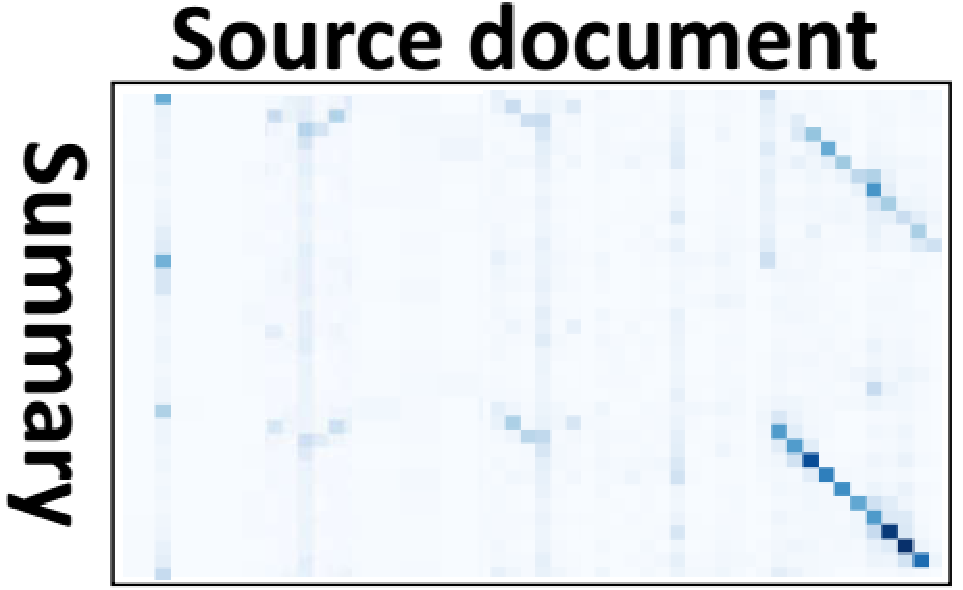
\includegraphics[width=0.16\linewidth]{mapITA}
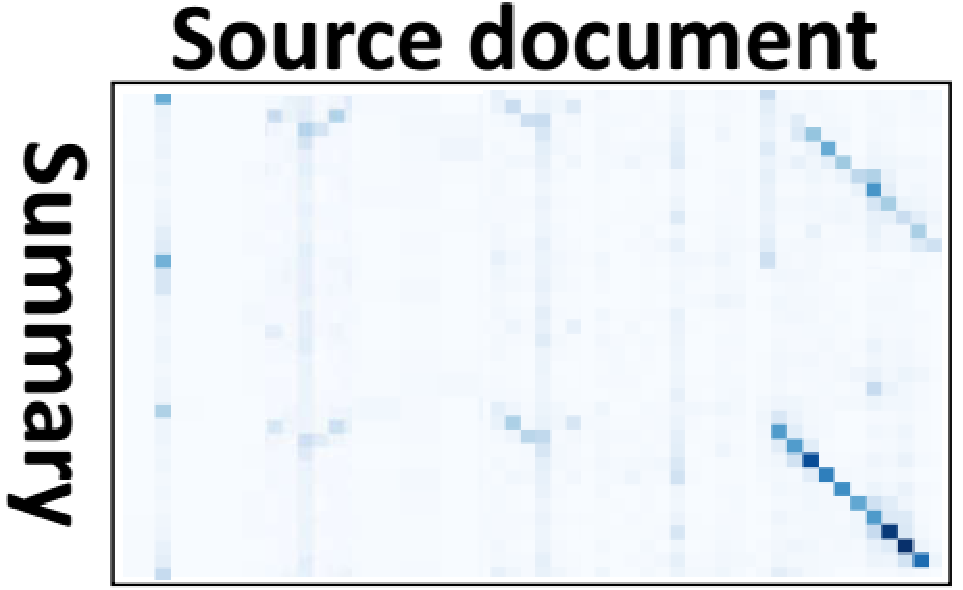
\includegraphics[width=0.26\columnwidth]{mapITA}
}
\quad
\subfigure[ITDA]{
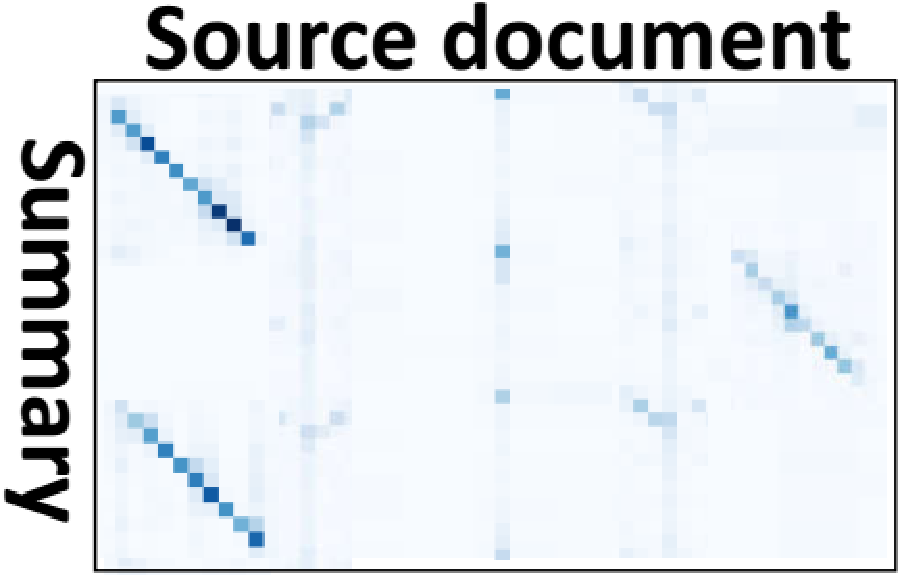
\includegraphics[width=0.26\linewidth]{mapITDA}
}
\quad
\subfigure[COV]{
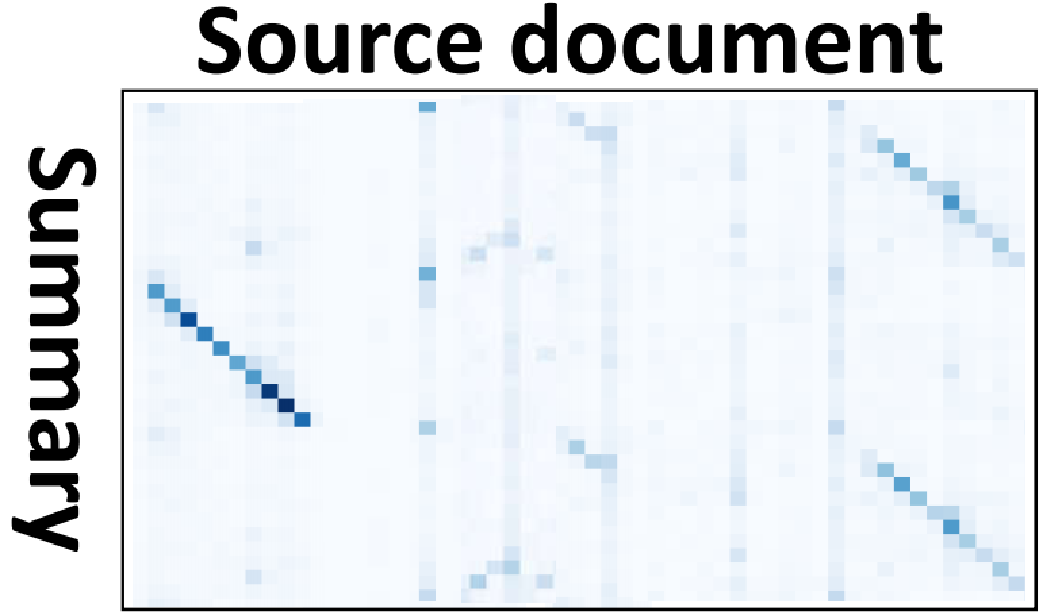
\includegraphics[width=0.26\linewidth]{mapCOV}
}
\quad
\subfigure[COVP]{
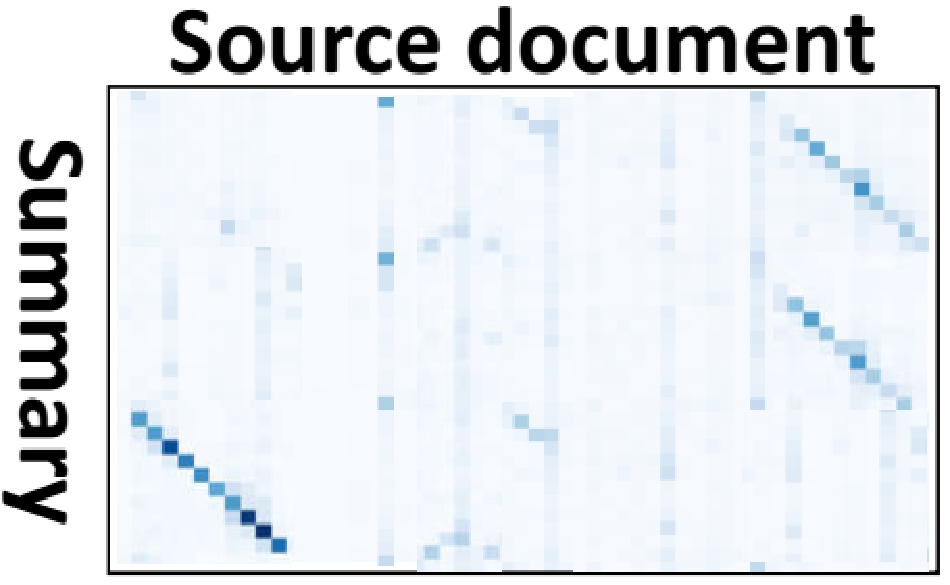
\includegraphics[width=0.26\linewidth]{mapCOVP}
}
\quad
\subfigure[SCL]{
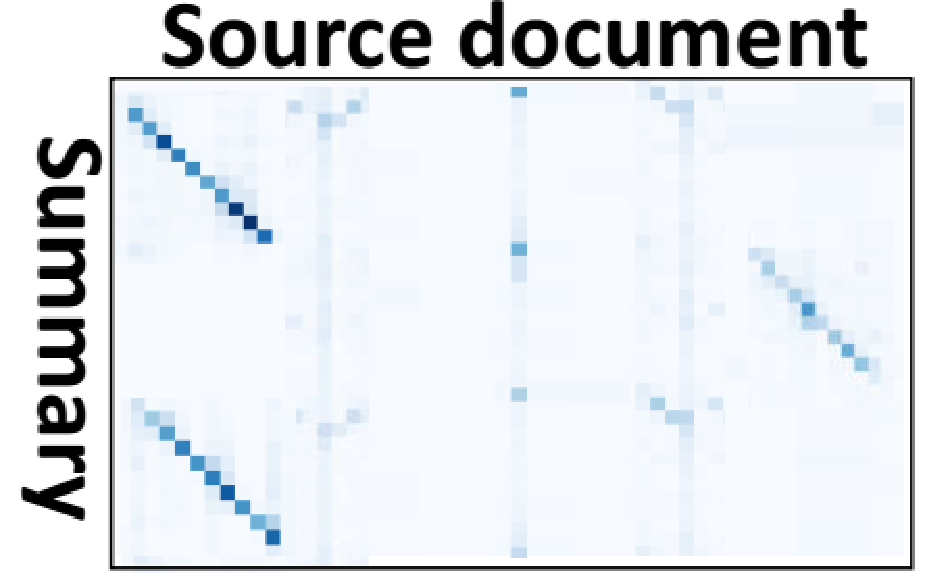
\includegraphics[width=0.26\linewidth]{mapSCL}
}
\quad
\subfigure[ATTF]{
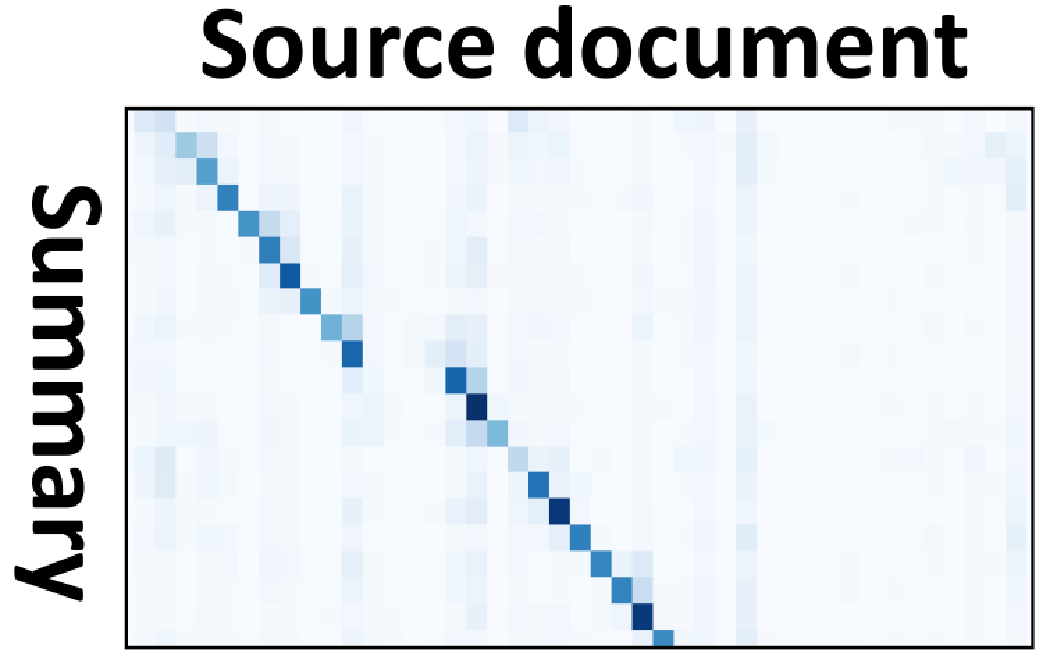
\includegraphics[width=0.26\linewidth]{map2}
}
%\caption{Attention distribution of examples in \tabref{tab:strong_methods}}
\caption{Attention distribution of summaries for the source in \tabref{tab:example}}
\label{fig:attn_maps}
\end{figure}

Compared with the Gold standard,
ATTF still generates some repetitive sentences,
due to similar sentences in source
such as \exref{ex:repeatsrc}.
%The result of summarizing that document using ATTF and its local attention map are
The summary generated by ATTF and its local attention are
shown in \tabref{tab:src_rep} and \figref{fig:attn_map3}.
Also, SBD further reduces the repetition when combined with ATTF. 
%which demonstrates its effectiveness.

\begin{table}[th!]
\begin{center}
\scriptsize
\begin{tabular}{|l|}%{|p{7cm}|rl|}
\hline \textbf{Reference:} oriol romeu is on a season-long loan at stuttgart from chelsea . \\
       the spanish midfielder predicts the scores in saturday 's matches . oriol goes \\
	   head-to-head with sportsmail 's martin keown .\\
\hline \textbf{ATTF:} chelsea beat manchester united on saturday . \textit{oriol romeu is currently} \\
       \textit{on a season-long loan at stuttgart . oriol romeu is currently on a season-long} \\
	   \textit{loan at bundesliga side stuttgart .}\\
\hline \textbf{SBD:} chelsea beat manchester united on saturday . chelsea face manchester \\
       united in the premier league . \\ 
\hline \textbf{ATTF+SBD:} chelsea face manchester united in the premier league on saturday . \\
       oriol romeu is currently on loan at stuttgart . \\
\hline
\end{tabular}
\end{center}
\caption{Summaries generated from \exref{ex:repeatsrc}.}
\label{tab:src_rep}
\end{table}

\begin{figure}[th!]
\centering
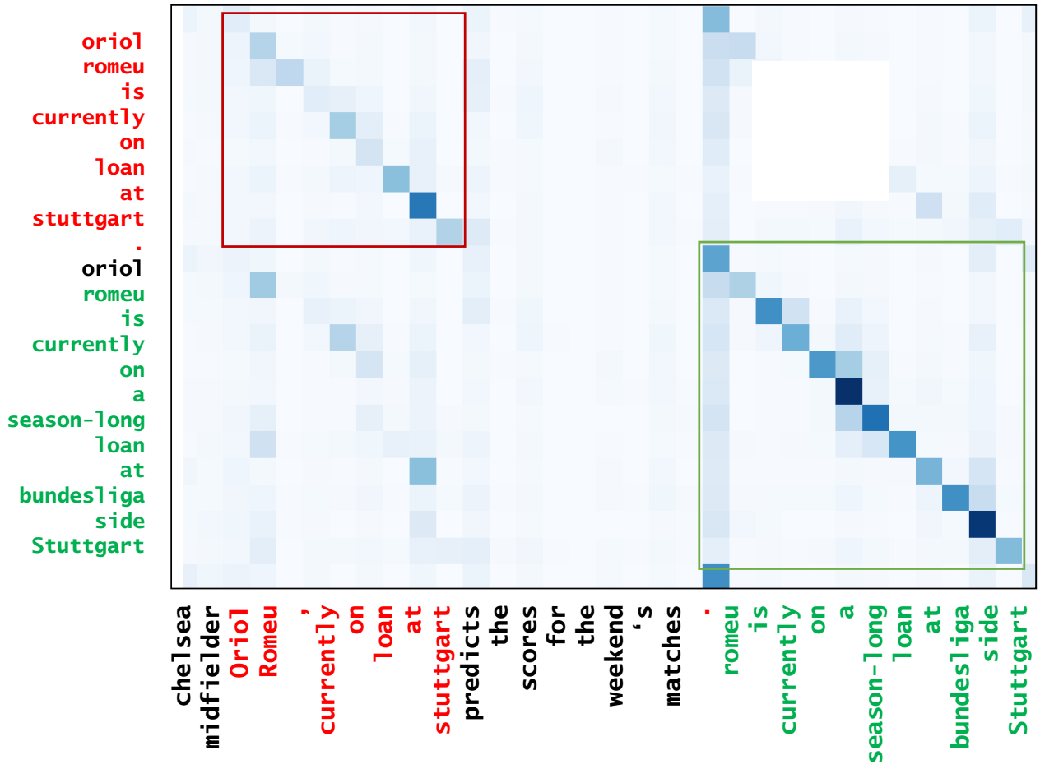
\includegraphics[width=0.84\columnwidth]{map3}
\caption{Attention distribution for ATTF in \tabref{tab:src_rep}}
\label{fig:attn_map3}
\end{figure}

As shown in \tabref{tab:eval_repe}, TRI has the lowest total repeatedness score.
It does not generate any repetitive N-grams (N$>$2) and sentences 
because TRI prevents the generation of the same trigrams during testing.
But as the Gold row shows, reference summaries do have some natural repetition.
%As reference summaries are human written, 
Therefore we evaluate the correlation of repeatedness distribution between
generated summaries and reference summaries (\tabref{tab:eval_repcor}).
Our proposed models achieve better results, among which ATTF+SBD performs best, an indication that ATTF and SBD are more capable of producing summaries with a natural level of repeatedness.
%It indicates that ATTF and SBD are more capable of producing summaries with a natural level of repeatedness.
%missing POIs and repetition in source documents.

\textbf{Readability.}
\DIFdelbegin \DIFdel{The readability scores of generated summaries are 
}\DIFdelend \DIFaddbegin \DIFadd{As }\DIFaddend shown in \tabref{tab:eval_repe}\DIFdelbegin \DIFdel{.
ATTF achieves the
}\DIFdelend \DIFaddbegin \DIFadd{, 
the models with ATTF achieve the
%DIF > ATTF achieves the
}\DIFaddend highest readability score among all baselines\DIFdelbegin \DIFdel{without 
any operations during testing.
}\DIFdelend \DIFaddbegin \DIFadd{, 
which means ATTF is more readable.
%DIF > without any operations during test.
}\DIFaddend TRI achieves the best score on repeatedness, 
% which represents the repetition over N-gram and sentences,
but lower readability score than other models.
Also, the readability of ATTF drops after adding TRI.
%All of our models score higher than $0.80$. 
SBD enhances performance of CNN and ATTF by reducing the repetitive unreadable sentences. 
ATTF+SBD scores highest on readability.

\begin{table}[th!]
	\centering
	\small
	\begin{tabular}{|l|c|c|c|}
		\hline
		     & pearson  & spearman & kendall's tau \\
		\hline
		TRI* & 1.0 & 0.894 & 0.837  \\
		SBD* & 1.0 & 1.0 & 1.0 \\
		%ATTF & 0.998 & 0.943 & 0.867 \\
		ATTF+TRI* & 1.0 & 0.894 & 0.837 \\
		ATTF+SBD* & \bf 1.0 & \bf 1.0 & \bf 1.0 \\
		\hline
	\end{tabular}
    \caption{Repeatedness correlation between generated summaries and Gold summaries.}
	\label{tab:eval_repcor}
\end{table}

\textbf{Speed.} 
As shown in \tabref{tab:eval_main} and \tabref{tab:eval_speed}, 
SBD is the best sentence-level backtracking decoder.
Compared with SBD-b1 and SBD-b2,
SBD logs higher ROUGE score without losing much on speed. 
We compare the speed of our model to RNN~\cite{SeeLM17} and FastRNN~\cite{P18-1063}
which used K40. 
We perform experiments on GTX-1080ti and scale the speed 
reported for the RNN methods,
since GTX-1080ti is twice as fast as K40~\cite{gehring2017convs2s}.
Our model can 
generate summaries much faster than previous RNN seq2seq models.
%FastRNN is also fast because 
\begin{table}[th!]
\centering
\small
\begin{tabular}{|l|c|c|c|}
\hline
Model & Time (s) & summaries/s & tokens/s \\
\hline
RNN  &  21600 & 0.48 & 29.60 \\
FastRNN &  3600 & 2.92 & 219.60 \\
\hline
CNN &  346.1 & 30.36 & 1343.46 \\
SBD-b1 &  412.8 & 25.46 & 1126.38 \\
SBD-b2 &  843.5 & 12.16 & 551.24 \\
SBD &  912.8 & 11.51 & 493.68 \\
ATTF & 1332 & 7.89 &  349.00 \\
ATTF+SBD & 1832.3 & 5.74 &  253.77 \\
\hline
\end{tabular}
\caption{Testing time and speed of generation.}
\label{tab:eval_speed}
\end{table}

%\subsection{Significance Test on ROUGE scores}

\textbf{Significance Test.} We use significance test to prove that the ROUGE scores in \tabref{tab:eval_main} is reliable.
We take Kruskal-Wallis test \cite{loukina2014automatic,albert2017exploring} as our
significance test to measure that the ROUGE scores
are significant or not. As shown in \tabref{tab:pvalue}, all p-values are less than 0.05. 
The smaller p-value, the higher significant.
Thus, the difference of the similarity results is significant. 
%\YZ{table for significance test}

\begin{table}[th]
	\small
	\centering
	\begin{tabular}{|c|c|c|}
		\hline
		R-1 & R-2 & R-L \\ \hline
		3.41e-32 & 2.12e-45 & 5.32e-12  \\ 
		\hline
	\end{tabular}
	\caption{p-value of significance test}
	\label{tab:pvalue}
\end{table}

The summaries generated by sequence-to-sequence models with attention mechanism always contain repetition.  
Through our observations, there are two reasons for repetition in abstractive summarization.
One is that the traditional attention mechanisms attend to the same location in source document at decoding.
The other is that the attention mechanism attend to the repetitive sentences in different locations in source document. 
As shown in \figref{fig:attn_maps} and \tabref{tab:src_rep},
our proposed ATTF and SBD effectively solve above two problems.  
The higher ROUGE scores (\tabref{tab:eval_main}) of our model means that
the summaries generated by our model are more similar to their corresponding reference summaries.
The natural-level repeatedness and higher readability score (\tabref{tab:eval_repe}) of our model means 
that our model can produce higher quality summaries\DIFaddbegin \DIFadd{.
Thus, our model can improve the reading speed and accuarcy of reading comprehension}\DIFaddend .


